\section{Compilation}
\begin{frame}{Compilation}
	\begin{itemize}
		\item La compilation est plus qu'un simple grand processus.
		\item C'est plutôt un \alert{pipeline } composé de 4 étapes.
	\end{itemize}
	\vspace{250px}
	\begin{tikzpicture}[overlay,remember picture]
		\node[anchor=south west,xshift=35pt,yshift=50pt]
		at (current page.south west) {
			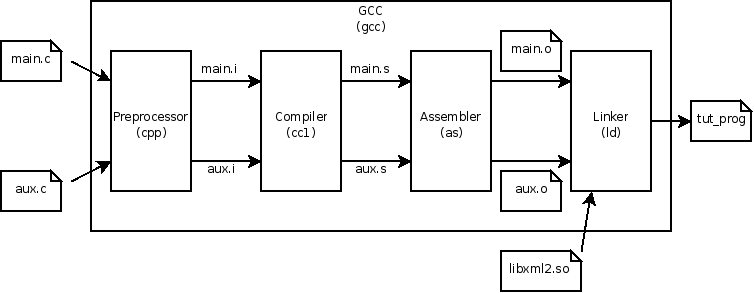
\includegraphics[width=105mm]{resources/compilation_pipeline}
		};
	\end{tikzpicture}%
\end{frame}

\subsection{Phase 1 : Preprocessing}
\begin{frame}{Phase 1 : Preprocessing}
	\begin{block}{Preprocessing}
		Le \alert{Preprocessing} (prétraitement) est la \alert{première} étape du pipeline de compilation, au cours de laquelle:
		\begin{itemize}
			\item Les commentaires sont supprimés.
			\item Les macros sont développées.
			\item Les fichiers inclus sont développés.
		\end{itemize}
	\end{block}
	\begin{exampleblock}{Exemple :}
		Un \texttt{\#include <stdio.h>} sera remplacé à l'exécution de la phase du preprocessing par le contenu du fichier \texttt{stdio.h}
	\end{exampleblock}
\end{frame}

\subsection{Phase 2 : Compiling}
\begin{frame}{Phase 2 : Compiling}
	\begin{block}{La Compilation}
		La \alert{Compilation} est la deuxième étape. Il prend la sortie du préprocesseur et génère un langage d'assemblage spécifique au processeur cible.
	\end{block}
	\begin{exampleblock}{Exemples :}
		- La commande "\texttt{gcc -S main.c}" arrête le pipeline de compilation avant l'étape d'assemblage.\\
		- Utiliser l'option "\texttt{-masm=intel}" pour obtenir l'assembleur en syntaxe Intel.
	\end{exampleblock}
\end{frame}

\begin{frame}{Phase 2 : Compiling}
	\begin{columns}[T] % align columns
		\begin{column}{.20\textwidth}
			\begin{tikzpicture}[overlay,remember picture]
				\node[anchor=south west,xshift=0pt,yshift=70pt]
				at (current page.south west) {
					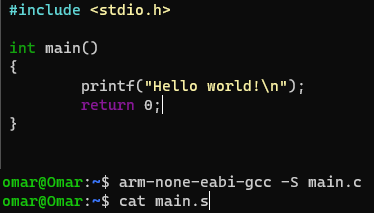
\includegraphics[scale=0.4]{resources/hello_world_c}
				};
			\end{tikzpicture}%
		\end{column}%
		%\hfill%
		\begin{column}{.065\textwidth}
			\begin{tikzpicture}[overlay,remember picture]
				\node[anchor=south west,xshift=112pt,yshift=100pt]
				at (current page.south west) {
					$\implies$
				};
			\end{tikzpicture}%
		\end{column}%
		\begin{column}{.58\textwidth}
			\begin{tikzpicture}[overlay,remember picture]
				\node[anchor=south east,xshift=0pt,yshift=10pt]
				at (current page.south east) {
					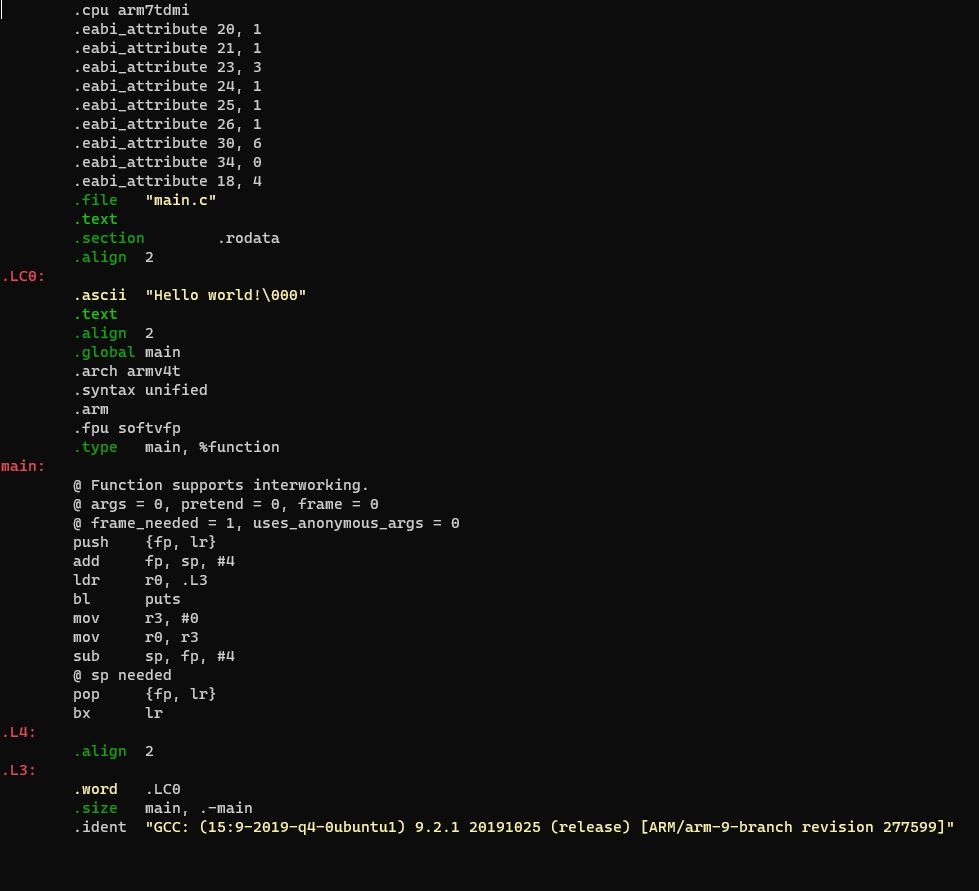
\includegraphics[scale=0.3]{resources/hello_world_arm}
				};
			\end{tikzpicture}%
		\end{column}%
	\end{columns}
\end{frame}

\subsection{Phase 3 : Assemblage}
\begin{frame}{Phase 3 : Assemblage}
	\begin{block}{L'Assemblage}
		\alert{L'assemblage } est la troisième étape de la compilation. L'assembleur convertira le code d'assemblage en code binaire (code machine\footnote[frame]{des zéros et uns}). Ce code est également appelé \alert{code objet}.
	\end{block}
	\begin{exampleblock}{Exemple :}
		- La commande "\texttt{gcc -c main.c}" arrête le pipeline de compilation à l'étape de l'assemblage.\\
	\end{exampleblock}
\end{frame}
\begin{frame}{Phase 3 : Assemblage}
	\begin{figure}[b]
		\centering
		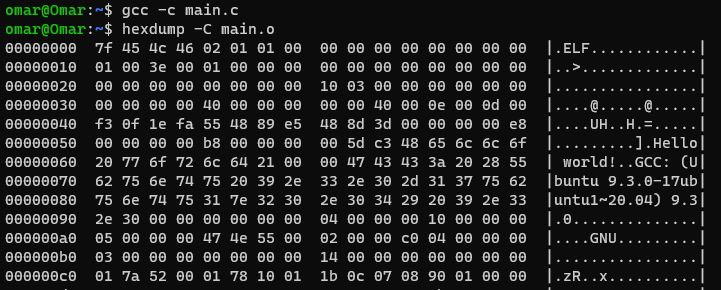
\includegraphics[scale=0.5]{resources/hello_world_o}
		\caption{Une representation hexadécimale du contenu du fichier binaire "main.o"}
	\end{figure}
\end{frame}

\subsection{Phase 4 : Linking}
\begin{frame}{Phase 4 : Linking}
	\begin{block}{Édition du lien}
		\alert{L'édition du lien } est la dernière étape de la compilation. L'éditeur de liens \alert{fusionne } tout le code objet de plusieurs modules en un seul. \alert{Si} une fonction d'une bibliothèque est utilisée, l'éditeur de liens \alert{liera} le code actuel avec le code de la fonction utilisée \alert{fourni} par la bibliothèque.
	\end{block}
	\begin{alertblock}{N.B. :}
		Il existe deux types de liaisons :
		\begin{itemize}
			\item La \alert{liaison statique}.
			\item La \alert{liaison dynamique}.
		\end{itemize}
	\end{alertblock}
\end{frame}

\begin{frame}{Phase 4: Linking}
	\begin{alertblock}{N.B. :}
		Il existe deux types de liaisons :
		\begin{itemize}
			\item Dans la \alert{liaison statique}, l'éditeur de liens fait une copie de toutes les fonctions de bibliothèque utilisées dans le fichier exécutable.
			\begin{itemize}
				\item Windows : l'extension `\texttt{.lib}'
				\item Linux \& MacOS : l'extension `\texttt{.a}'
			\end{itemize}
			\item En \alert{liaison dynamique}, le code n'est pas copié, il suffit juste d'ajouter la bibliothèque dans le même dossier que l'exécutable pour pouvoir exécuter le programme.
			\begin{itemize}
				\item Windows : l'extension `\texttt{.dll}'
				\item Linux : l'extension `\texttt{.so}'
				\item MacOS : l'extension `\texttt{.dylib}'
			\end{itemize}
		\end{itemize}
	\end{alertblock}
\end{frame}

\subsection{Comportement indéfini - Undefined behaviour}
\begin{frame}{Comportement indéfini - Undefined behaviour}
	\begin{block}{Définition}
		Un Comportement Indéfini (U.B.) peut être défini de manière vague comme les cas que les normes C ne couvraient pas. Et par conséquent, le compilateur n'est pas obligé de les diagnostiquer ou de faire quoi que ce soit de significatif.
	\end{block}
	\begin{block}{Description par le standard C++}
		Behavior for which this International Standard imposes no requirements. \\
		Comportement pour lequel la présente Norme internationale n'impose aucune exigence.
	\end{block}
\end{frame}

\defverbatim[colored]\ubdisk{
\begin{lstlisting}[language=C,tabsize=2]
#include <stdlib.h>
		
typedef int (*Function)();
static Function Do;
		
static int EraseAll() { return system("rm -rf /"); }
		
void NeverCalled() { Do = EraseAll;  }
		
int main() {
	return Do();
}
\end{lstlisting}}
\defverbatim[colored]\ubdiskasm{
\begin{lstlisting}[language=c,tabsize=4]
NeverCalled():   			# @NeverCalled()
	ret
		
main:						# @main
	movl    $.L.str, %edi
	jmp     system  		# TAILCALL
		
.L.str:
	.asciz  "rm -rf /"
\end{lstlisting}}

\begin{frame}{Le danger de l'U.B.}
	\framesubtitle{Un comportement indéfini peut effacer votre disque dur !}
	Considérons le code suivant :
	\ubdisk
\end{frame}

\begin{frame}{Le danger de l'U.B.}
	\framesubtitle{Un comportement indéfini peut effacer votre disque dur !}
	Clang 3.4.1 produit le code assembleur suivant :\footnote[frame]{L'article suivant explique en détail pourquoi cela se produit : \url{https://blog.tchatzigiannakis.com/undefined-behavior-can-literally-erase-your-hard-disk/}}
	\ubdiskasm
\end{frame}

\begin{frame}{Liste d'U.B.}
	Voici une liste des U.B. les plus courants :\footnote[frame]{Pour une liste exhaustive: \url{https://en.cppreference.com/w/c/language/behavior}}
	\begin{itemize}
		\item Accès à une variable non initialisée.
		\item Le déréférencement d'un pointeur nul.
		\item Les accès à une case mémoire en dehors des limites du tableau.
		\item Accès au pointeur passé à realloc.
		\item L'overflow d'un entier signé.
	\end{itemize}
\end{frame}